\begin{figure}[t]
\centering
\scriptsize
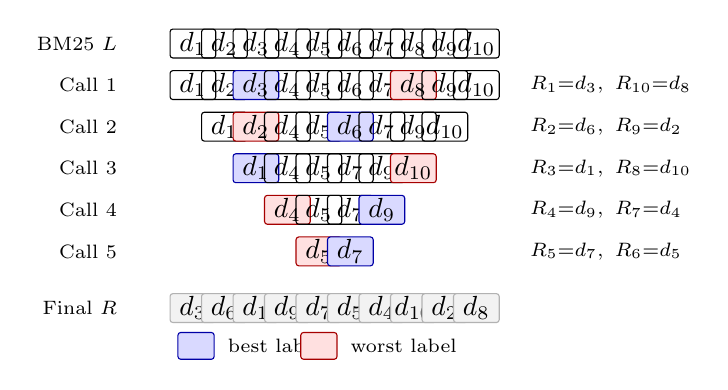
\begin{tikzpicture}[
  x=0.40cm,
  y=0.48cm,
  doc/.style={draw, rounded corners=1pt, minimum width=0.58cm, minimum height=0.34cm, inner sep=1pt},
  best/.style={doc, fill=blue!15, draw=blue!65!black},
  worst/.style={doc, fill=red!12, draw=red!65!black},
  placed/.style={doc, fill=gray!10, draw=gray!60},
  label/.style={anchor=east, font=\scriptsize},
  note/.style={anchor=west, font=\scriptsize}
]

\node[label] at (-1.1,0) {BM25 $L$};
\foreach \d [count=\i from 1] in {1,2,3,4,5,6,7,8,9,10} {
  \node[doc] at (\i,0) {$d_{\d}$};
}

\node[label] at (-1.1,-1.1) {Call 1};
\foreach \d [count=\i from 1] in {1,2,3,4,5,6,7,8,9,10} {
  \ifnum\d=3
    \node[best] at (\i,-1.1) {$d_{\d}$};
  \else
    \ifnum\d=8
      \node[worst] at (\i,-1.1) {$d_{\d}$};
    \else
      \node[doc] at (\i,-1.1) {$d_{\d}$};
    \fi
  \fi
}
\node[note] at (11.4,-1.1) {$R_1{=}d_3,\ R_{10}{=}d_8$};

\node[label] at (-1.1,-2.2) {Call 2};
\foreach \d [count=\i from 1] in {1,2,4,5,6,7,9,10} {
  \ifnum\d=6
    \node[best] at (\i+1,-2.2) {$d_{\d}$};
  \else
    \ifnum\d=2
      \node[worst] at (\i+1,-2.2) {$d_{\d}$};
    \else
      \node[doc] at (\i+1,-2.2) {$d_{\d}$};
    \fi
  \fi
}
\node[note] at (11.4,-2.2) {$R_2{=}d_6,\ R_9{=}d_2$};

\node[label] at (-1.1,-3.3) {Call 3};
\foreach \d [count=\i from 1] in {1,4,5,7,9,10} {
  \ifnum\d=1
    \node[best] at (\i+2,-3.3) {$d_{\d}$};
  \else
    \ifnum\d=10
      \node[worst] at (\i+2,-3.3) {$d_{\d}$};
    \else
      \node[doc] at (\i+2,-3.3) {$d_{\d}$};
    \fi
  \fi
}
\node[note] at (11.4,-3.3) {$R_3{=}d_1,\ R_8{=}d_{10}$};

\node[label] at (-1.1,-4.4) {Call 4};
\foreach \d [count=\i from 1] in {4,5,7,9} {
  \ifnum\d=9
    \node[best] at (\i+3,-4.4) {$d_{\d}$};
  \else
    \ifnum\d=4
      \node[worst] at (\i+3,-4.4) {$d_{\d}$};
    \else
      \node[doc] at (\i+3,-4.4) {$d_{\d}$};
    \fi
  \fi
}
\node[note] at (11.4,-4.4) {$R_4{=}d_9,\ R_7{=}d_4$};

\node[label] at (-1.1,-5.5) {Call 5};
\foreach \d [count=\i from 1] in {5,7} {
  \ifnum\d=7
    \node[best] at (\i+4,-5.5) {$d_{\d}$};
  \else
    \node[worst] at (\i+4,-5.5) {$d_{\d}$};
  \fi
}
\node[note] at (11.4,-5.5) {$R_5{=}d_7,\ R_6{=}d_5$};

\node[label] at (-1.1,-7.0) {Final $R$};
\foreach \d [count=\i from 1] in {3,6,1,9,7,5,4,10,2,8} {
  \node[placed] at (\i,-7.0) {$d_{\d}$};
}

\node[best, minimum width=0.46cm] at (1.1,-8.0) {};
\node[note] at (1.8,-8.0) {best label};
\node[worst, minimum width=0.46cm] at (5.0,-8.0) {};
\node[note] at (5.7,-8.0) {worst label};
\end{tikzpicture}
\caption{A ten-document run fills the ranking from both ends as the live pool shrinks.}
\label{fig:dualend}
\end{figure}
